\documentclass[10pt,twocolumn,letterpaper]{article}
\usepackage[T1]{fontenc}
\usepackage[review,applications]{wacv}
\usepackage{graphicx}
\usepackage{booktabs}
\usepackage{amsmath,amssymb}
\usepackage{microtype}
\definecolor{wacvblue}{rgb}{0.21,0.49,0.74}
\usepackage[pagebackref,breaklinks,colorlinks,allcolors=wacvblue]{hyperref}
\def\wacvPaperID{DRAFT}
\def\confName{WACV}
\def\confYear{2027}
\title{Evaluating Learned Skeleton Features in Neurological Gait Videos}
\author{Anonymous submission}
\begin{document}
\maketitle
\begin{abstract}
Video-based gait analysis could support research on neurological movement, but a classifier may use average posture or recording conditions as well as movement over time. We test whether learning from sequences of automatically tracked body landmarks improves on a simple average-pose summary. The collection contains 88 usable clips from 41 source recordings, labeled Normal, multiple sclerosis, or Parkinson's disease; these labels were not clinically verified. A skeleton joint-embedding predictive architecture (S-JEPA) learns numerical descriptions of the clips by predicting hidden features. We keep source recordings separate during training, model selection, and testing, and compare the learned descriptions with simpler summaries. Macro-F1, which averages F1 across the three labels, is 0.457 for S-JEPA and 0.452 for mean pose when every source recording receives equal total weight. Resampling whole sources gives a difference of 0.005 with a conditional 95\% interval of $[-0.160,0.174]$. Mean pose performs better when clips receive equal weight and in four of five test groups. These results leave the advantage over mean pose unresolved. Unverified participant identities and a mismatch between reflection and training masks further limit interpretation. The study illustrates the value of simple pose summaries and explicit evaluation units when assessing learned gait features.
\end{abstract}

\section{Introduction}
Changes in walking are relevant to the study of neurological disease, yet their expression varies between people and conditions. Clinical studies have described heterogeneous walking dysfunction in multiple sclerosis (MS), including changes in bilateral coordination~\cite{filli2018,plotnik2020}. Video-based measurements could make movement analysis more accessible, provided that the relationship between recorded motion, extracted pose, and the intended clinical measurement is established. Validation studies of video-derived gait measures~\cite{stenum2021,stenum2024} and work on Parkinson's disease (PD)~\cite{shin2021} motivate this direction without validating every subsequent classifier trained on video.

Learning from heterogeneous recordings introduces another difficulty. A pose sequence contains body configuration and changes over time, but also measurement effects associated with viewpoint, occlusion, and the pose estimator. Several clips may come from the same source video. A representation can consequently predict a collection label through cues that will not transfer to a new recording setting. Source-separated evaluation and informative simple baselines help assess this possibility, even when the available metadata cannot establish participant independence.

We investigate whether a model that learns numerical summaries of skeleton sequences provides a consistent classification advantage over simple pose averages in a small collection labeled Normal, MS, and PD. The feature-extraction network, or encoder, follows the joint-embedding predictive approach developed for images, video, and skeletons~\cite{ijepa,vjepa,sjepa}, with stochastic masking of body regions and label-free training on the training sources. After this training, the encoder is held fixed. A separate linear classifier combines its features to predict the three collection labels.

The empirical contribution is a bounded comparison: the learned model's small overall lead over mean pose reverses when clips, rather than source recordings, receive equal weight. The learned model leads in only one of the five test groups. We compare both methods and a visibility-only summary on the same source partitions, so readers can assess the extent and consistency of the differences. This makes the study relevant to behavioral phenotyping from markerless pose: it examines what a small video collection can support before the output is interpreted as a clinical measure. It contains no neural recordings or direct neural decoding experiment.

\section{Related work}
Video-based gait analysis has been evaluated against reference measurements and across clinical populations~\cite{stenum2021,stenum2024}. Such studies assess defined movement quantities under specified conditions. Our outcome is instead a supplied video label, with no independently verified diagnosis or reference kinematics. The difference in supervision matters when comparing conclusions across these settings.

Skeleton representation learning includes masked reconstruction and motion pretraining, as illustrated by SkeletonMAE and MotionBERT~\cite{skeletonmae,motionbert}. I-JEPA and V-JEPA predict learned target features from context~\cite{ijepa,vjepa}; S-JEPA applies a joint-embedding predictive architecture to skeleton sequences~\cite{sjepa}. The original S-JEPA samples target joints with probabilities related to motion. Our compact adaptation uses video-derived 2D coordinates and visibility, with masks sampled from body regions. This sampling choice is motivated by gait anatomy. The study does not isolate the effect of that rule or establish a new general-purpose skeleton-learning method.

Small-sample model evaluation can have large uncertainty, and using the same data for model selection and evaluation can bias the reported error~\cite{varoquaux2018,varma2006}. We therefore separate training, validation, and outer-test sources. This controls source overlap within the specified evaluation procedure, although it cannot account for every decision made during development on this collection.

\begin{figure*}[t]
\centering
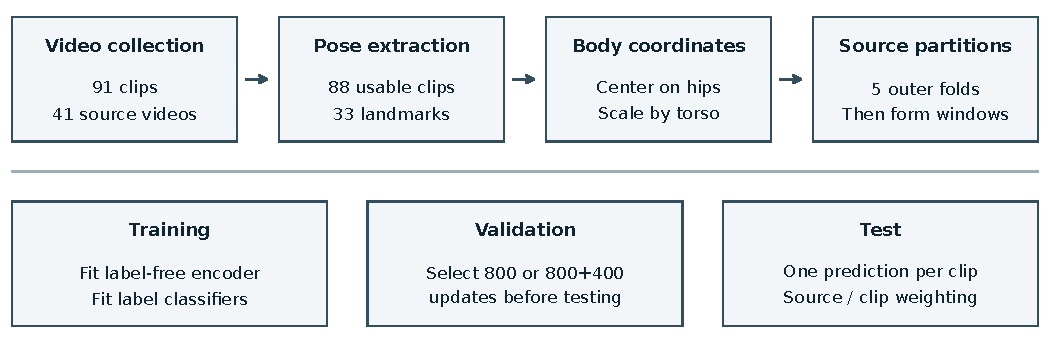
\includegraphics[width=\textwidth]{figures/pipeline-v5.pdf}
\caption{The notebook-defined evaluation. Pose extraction precedes body-relative normalization. Source partitions are fixed before window generation; encoder training and label-classifier fitting use only training sources, and validation chooses the training stage. Test predictions are pooled under two explicitly defined weighting rules.}
\label{fig:pipeline}
\end{figure*}

\section{Video collection and pose processing}
The collection contains 91 downloaded MP4 clips grouped by an 11-character source-video identifier. The labels Normal, MS, and PD describe collection metadata, not diagnoses established by this study. Pose cleaning retains 88 clips from 41 sources (Table~\ref{tab:data}). A source identifier is a recording identifier: different sources may contain the same participant, while one source may contain more than one person. Neither possibility is resolved by the available metadata.

\begin{table}[t]
\centering
\caption{Collection composition. A padded clip has fewer than 32 retained frames. Windows overlap within a clip and are not independent observations.}
\label{tab:data}
\small
\setlength{\tabcolsep}{4pt}
\begin{tabular}{lrrrrr}
\toprule
Label & Raw & Usable & Sources & Padded & Windows\\
\midrule
Normal &26&24&16&5&59\\
MS &30&29&13&0&171\\
PD &35&35&12&10&128\\
\midrule
Total &91&88&41&15&358\\
\bottomrule
\end{tabular}
\end{table}

The extraction pipeline uses MediaPipe pose estimation from the BlazePose family~\cite{blazepose}. It processes full frames and retains the first detected pose. The cached array has 33 landmarks with pixel $x$, pixel $y$, and a visibility value for each sampled frame. Visibility is the detector's estimate of whether a landmark is visible; it is neither a clinical confidence score nor an independently measured quality rating. The pose-estimator interface converts its image-normalized coordinates to pixels before caching; the subsequent body-relative normalization described below is a separate operation. Depth is not used.

Frames are selected with integer stride $\max(1,\operatorname{round}(f_{\rm src}/15))$. Thus, 15 frames per second is a nominal target rather than an exact common sampling rate. Windows contain the same number of sampled frames but can cover different lengths of time. Cleaning requires finite $x$ coordinates for every landmark in at least 30\% of sampled frames, trims empty ends, and interpolates missing coordinates and visibility within the sequence. No maximum interior gap length is imposed. At least eight frames must survive cleaning. Three clips are excluded, but the saved exclusion list does not identify a separate failure criterion for each.

For pixel position $x_{tj}\in\mathbb{R}^2$, hip midpoint $h_t$, and shoulder midpoint $s_t$, the normalized coordinates are
\begin{equation}
\widetilde{x}_{tj}=\frac{x_{tj}-h_t}{\max(\|s_t-h_t\|_2,10^{-3})}.
\label{eq:normalization}
\end{equation}
Spatial normalization leaves the already cleaned visibility values unchanged. This transformation removes absolute pelvis translation and apparent torso size. Within each frame it preserves defined angles under a common positive scale, but frame-varying scale changes displacement over time. The resulting trajectories are not calibrated measurements of physical speed or stride length.

Each source is assigned to a partition before generating 32-frame windows with stride 16. A shorter clip is padded by repeating its final frame. There are 358 windows in total, including 15 padded clips. Padding and interpolation can change apparent dynamics. Table~\ref{tab:data} reports the padding counts by label; the retained caches do not provide per-label counts or gap lengths for interpolation.

\section{Predictive skeleton representation}
\subsection{Stochastic region masking}
A training window contains all 33 landmarks and three channels. Four consecutive frames for one landmark form a token, giving eight time blocks and $8\times33=264$ tokens. The masking sampler operates on seven overlapping regions: head, mouth, left arm, right arm, trunk, left leg, and right leg. It draws one region and a contiguous span of one to six time blocks, adds their tokens to the target set, and repeats until it reaches the rounded target budget of 158 tokens (nominally 60\%) or a 36-draw guard. Span length and admissible start position are drawn uniformly. Region overlap and the final draw mean the realized target fraction can exceed 60\%.

Twelve landmarks influence region-selection weights: both shoulders, hips, knees, ankles, heels, and foot indices. A region containing any of these landmarks receives a factor of 1.5, divided by the average number of regions containing its constituent joints; the resulting weights are normalized over regions. This is a bias in region selection. It neither fixes which joints are masked nor makes each highlighted joint 1.5 times as likely to be hidden. Shoulders and hips appear in two regions, so the overlap correction does not equalize their final masking frequencies.

The arms also receive the boost because they contain shoulders, so their elbows, wrists, and hand landmarks inherit that region weight. Every example receives a new mask. The sampler guarantees at least one visible token from the twelve-landmark set somewhere in the window, as well as nonempty target and context sets. The retained token can be a shoulder: neither hip nor leg context is guaranteed even somewhere in a particular window, and an entire time block can be hidden. In the notebook's separate seed-zero bank of 512 masks, the mean target fraction is 63.3\%, and every joint is visible somewhere in at least 74.0\% of windows. These sampler diagnostics describe draws from the rule, not realized exposure in the five-fold training run. The anatomical choice is a design hypothesis motivated by gait analysis. No comparison with uniform, motion-dependent, or alternative anatomical masking establishes its benefit.

\subsection{Learning to predict hidden features}
The encoder converts each group of four frames for one landmark into a 96-number feature vector. Learned position codes specify the landmark and time block. Transformer layers combine information across visible positions, and a second network predicts features at the hidden positions. A reference network, called the target encoder, supplies those training targets. It starts as a copy of the context encoder and is updated gradually toward its weights through an exponential moving average (EMA). This makes the targets change more slowly than the network being optimized. Table~\ref{tab:settings} records the architecture and optimization settings.

\begin{table}[t]
\centering
\caption{Settings for the evaluated model. Both training stages use the same architecture and loss; the continuation restarts optimization state.}
\label{tab:settings}
\small
\setlength{\tabcolsep}{4pt}
\begin{tabular}{p{.43\columnwidth}p{.49\columnwidth}}
\toprule
Setting & Value\\
\midrule
Input window & $32\times33\times3$\\
Frames per landmark token & 4 (12 input values)\\
Encoder / predictor depth & 3 / 2 transformer layers\\
Feature width / attention heads & 96 / 4\\
Feed-forward expansion / dropout & 2 / 0\\
Batch size / training updates & 32 / 800, then 400\\
AdamW peak rate / weight decay & $10^{-3}$ / 0.05\\
AdamW coefficients / norm clip & $(0.9,0.95)$ / 1\\
Learning-rate schedule & 10\% warmup, cosine decay\\
EMA momentum & Cosine, 0.996 toward 1\\
Center momentum & 0.9\\
Prediction / target temperature & 0.10 / 0.06\\
Initialization and training seed & 42\\
\bottomrule
\end{tabular}
\end{table}

The context network receives a geometrically transformed window. Rotation is sampled within $\pm15^\circ$, scale within $[0.9,1.1]$, and translation within $\pm0.1$ body-normalized units per axis. Horizontal reflection occurs with probability 0.5 and exchanges left and right landmark slots, including their visibility values. One transform applies to the whole window. To withhold the hidden observations, visible positions cannot draw information from target positions in the context encoder. The implementation enforces this through an attention mask and replaces hidden-position outputs with a shared learned placeholder before prediction. The predictor also receives joint and time position codes, so different hidden positions can receive different predictions. The target encoder receives the complete, untransformed window and changes only through weight averaging. The loss compares predicted and target distributions over the 96 feature dimensions at masked slots; these distributions are not class probabilities.

Training penalizes disagreement between predicted and reference features. Each 96-number vector is converted to nonnegative weights that sum to one, and cross-entropy measures how closely the two distributions agree. A running mean centers the reference features before this conversion; the temperature settings in Table~\ref{tab:settings} control how concentrated the distributions become. We first average the error over hidden positions within a window, then give each window equal weight in its batch. The running mean is updated once per batch from all masked reference vectors, so this centering step weights token positions equally. The exact equations and update rules appear in the companion methods record.

Training samples windows with replacement so that each training source has equal total probability. The batch size is 32, with 800 initial updates and a 400-update continuation on the same training sources. Both stages use all training sources and the same prediction task, without condition labels in the encoder loss. Continuation retains network weights but resets the optimizer, center, random streams, and schedules. It therefore differs from uninterrupted training for 1,200 updates.

The settings in Table~\ref{tab:settings} define the evaluated configuration. They do not describe an independently optimized architecture. The technical implementation, including the feature-distribution loss and its weighting, is recorded in the companion methods audit.

\subsection{From learned features to a clip label}
For classification, we keep the target encoder's weights fixed and supply every token of the complete window. We average its features at the 161 token positions selected by one fixed mask drawn with seed zero, then average window vectors within each clip. The mask here selects output positions; it does not hide the corresponding input coordinates. All 33 landmarks occur at least once in the selected positions. The result is one 96-dimensional vector per clip.

Each feature is standardized using training clips only, then a logistic-regression classifier is fitted to their labels ($C=1$, maximum 2,000 iterations, seed 42). This is a linear classifier: it combines the feature values with learned weights. Class weighting gives greater fitting weight to labels with fewer training clips. Each training stage has its own classifier. Validation source-weighted macro-F1 selects the stage, with ties retaining the initial stage; the chosen model is then applied to outer-test clips. The scaler, classifier, and encoder are not refit on combined training and validation sources. These class weights do not equalize recordings within a label: a source with many clips still has more influence on classifier fitting than a source with one clip.

\section{Evaluation}
\subsection{Partitions and baselines}
We sort the source identifiers and divide one row per source into five groups using shuffled, label-stratified splitting (\texttt{StratifiedKFold}). The procedure distributes the three labels across groups, then expands source assignments to clips. Each group serves once as the outer test set, or fold. Among the other sources, the first split from a four-fold version of the same procedure forms a separate validation group for choosing the training stage. The outer seed is 42 and the inner seed is $43+k$ for fold $k$. This gives five test evaluations, each with one validation group; we do not search across every possible inner split. Every retained clip has exactly one outer-test prediction.

\begin{table}[t]
\centering
\caption{Source/clip counts in the fixed partitions.}
\label{tab:splits}
\begin{tabular}{crrr}
\toprule
Fold & Training & Validation & Test\\
\midrule
0&24/51&8/19&9/18\\
1&24/58&9/17&8/13\\
2&24/54&9/17&8/17\\
3&24/53&9/21&8/14\\
4&24/45&9/17&8/26\\
\bottomrule
\end{tabular}
\end{table}

Mean pose averages normalized $x,y$ over each complete clip, yielding 66 features without temporal order. Visibility uses the mean and standard deviation of each landmark's visibility, also yielding 66 features. Both use the same linear-classifier recipe as the learned representation. Mean pose retains posture and viewing geometry, while visibility may reflect occlusion, body orientation, or detector behavior. Neither is a pure measurement of recording conditions.

The engineered-feature baseline reads cleaned pixel coordinates. Its intended vector contains six per-side hip, knee, and ankle angle means, three absolute bilateral mean differences, and six per-side ranges. The legacy container has 82 fields, but only 15 columns vary in each training fold along this extraction route. In the notebook-reported experiment, the left-ankle range duplicates the right-ankle range. This omits one intended measurement and limits conclusions about the intended baseline. Its Random Forest has 100 trees, maximum depth five, square-root feature subsampling, class-balanced training, and seed 42. Columns constant in the training partition are removed, and the remaining features are standardized using that partition. A majority-class baseline predicts the most frequent training-clip label in each fold. All methods use identical outer partitions, but the S-JEPA procedure additionally selects between two stages on validation data. These are comparisons of complete procedures: they do not isolate the effect of temporal information alone.

\subsection{Scoring}
F1 balances precision (how often a predicted label is correct) and recall (how many examples with that label are found). We calculate F1 separately for Normal, MS, and PD, then average the three values to obtain macro-F1. Higher values are better, with one representing perfect predictions; the score is not the fraction of correctly classified clips. Our primary descriptive measure gives every source recording equal total weight and combines all test predictions before scoring. We call this pooled source-weighted macro-F1. For example, each of the 13 clips from one MS source contributes weight $1/13$, while a clip from a source with only one clip contributes weight one. More generally, if source $s$ contributes $n_s$ clips, each clip receives weight $1/n_s$. For supplied label $a$ and prediction $b$, weighted confusion counts are
\begin{equation}
C_{ab}=\sum_i \frac{\mathbf{1}(y_i=a,\widehat{y}_i=b)}{n_{s(i)}}.
\end{equation}
The class F1 score is $2C_{aa}/(\sum_b C_{ab}+\sum_b C_{ba})$, and macro-F1 averages the three class values. Each source contributes total weight one before scoring. This is not an average of source-level F1 scores or a classification of one aggregated prediction per source.

We also report pooled clip-weighted macro-F1 and the mean and population standard deviation of the five source-weighted fold scores. Pooled F1 differs from the mean of fold F1 because the score is nonlinear. Fold standard deviation describes heterogeneity and is not a confidence interval; the folds have overlapping training sets. We assess sensitivity to the sampled sources by repeatedly drawing whole source videos, a procedure called a source bootstrap. It is a retrospective analysis of the notebook-associated test predictions. In each of 10,000 draws (seed 20261004), we sample 16 Normal, 13 MS, and 12 PD sources with replacement within each label group. Each sampled occurrence contributes total weight one, distributed equally among that source's clips, and every method uses the same source draws. We recompute pooled macro-F1 and paired differences, reporting the 2.5th and 97.5th percentiles.

The resulting intervals describe variation when sources are resampled while the fitted models, their predictions, and the number of sources per label remain fixed. They do not capture changes caused by retraining, another random initialization, different partitions, or other choices made during development. Sources are treated as independent clusters even though participant overlap is unresolved, and shared training data induce dependence across fitted outer-fold models. We use the intervals as descriptive sensitivity summaries, not a confirmatory population test or evidence of equivalence. This analysis was added for the manuscript; it is not a saved notebook output.

\section{Results}
Table~\ref{tab:results} reports the primary notebook-defined experiment, with scores checked against its 88 saved outer-test rows. S-JEPA reaches source-weighted macro-F1 0.457 and mean pose reaches 0.452, a difference of 0.0047. Under clip weighting their ordering reverses: mean pose reaches 0.410 and S-JEPA 0.397. Mean pose correctly classifies 37 clips and S-JEPA 36. One MS source contributes 13 clips, making the choice of weighting consequential.

\begin{table}[t]
\centering
\caption{Held-out macro-F1. Source and clip columns pool all outer-test predictions; the last column summarizes source-weighted fold scores. SD is descriptive. $^*$The notebook RF contains a duplicated ankle-range feature.}
\label{tab:results}
\small
\setlength{\tabcolsep}{4pt}
\begin{tabular}{lrrr}
\toprule
Representation & Source & Clip & Fold mean $\pm$ SD\\
\midrule
S-JEPA &0.457&0.397&$0.438\pm0.196$\\
Mean pose &0.452&0.410&$0.427\pm0.132$\\
Joint angles + RF$^*$ &0.411&0.397&$0.395\pm0.098$\\
Visibility &0.318&0.318&$0.285\pm0.104$\\
Majority class &0.259&0.202&$0.159\pm0.022$\\
\bottomrule
\end{tabular}
\end{table}

The conditional interval for S-JEPA macro-F1 is $[0.329,0.579]$. Its paired difference from mean pose is $0.0047$ with interval $[-0.160,0.174]$; against the notebook RF it is $0.0454$ with interval $[-0.133,0.220]$. Both span zero. The data and this conditional procedure leave the directions uncertain without showing that the methods are equivalent.

\begin{figure*}[t]
\centering
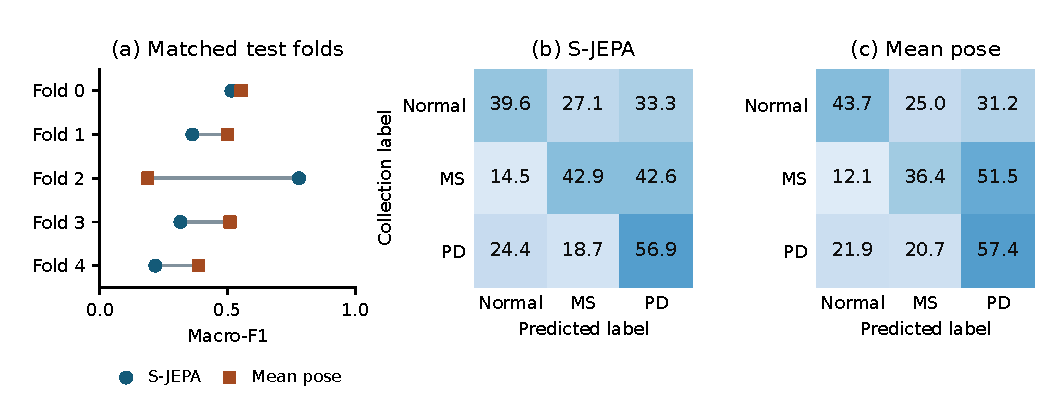
\includegraphics[width=\textwidth]{figures/folds-and-errors-v5.pdf}
\caption{Notebook-associated outer-test results. (a) Source-weighted macro-F1 in each test fold. A straight line joins the two methods evaluated on the same sources; circles denote S-JEPA and squares mean pose. (b,c) Row-normalized source-weighted confusion percentages. Rows are collection labels, columns predictions, and each source contributes total weight one before row normalization. These are not percentages of clinically verified patients.}
\label{fig:results}
\end{figure*}

Mean pose exceeds S-JEPA in four of five outer folds (Figure~\ref{fig:results}a). The pooled difference consequently does not describe a consistent foldwise improvement. The visibility-only score is lower than both coordinate-based representations, but this comparison cannot quantify how much recording information remains in their features. Mean pose retains average body configuration and can reflect time spent in different positions, even though it discards their order. Its competitiveness therefore does not imply that all movement-related information has been removed. S-JEPA fold scores range from 0.217 to 0.780. Its raw correct counts are 10/24 Normal, 8/29 MS, and 18/35 PD clips; source-weighted recalls are 0.396, 0.429, and 0.569 (Figure~\ref{fig:results}b). The average score therefore coexists with substantial errors in all three labels.

The initial stage is selected in folds zero through two, and continuation in folds three and four. The final training batch has lower prediction error after continuation in every fold, yet the validation classification score improves in only two. Lower error on that sampled batch therefore did not reliably identify the stage selected for classification. Because the endpoint batches differ, these values do not measure average prediction error on a common evaluation set.

The primary comparison follows the protocol and written results in the top-level notebooks. We verified these results against the matching saved predictions; the notebook's evaluation code has no saved cell outputs. The companion audit record (\texttt{evidence/reproducibility.md}) names the notebook-associated execution and separately identifies the corrected verification. It records input hashes and the command for \texttt{evidence/results\_audit.py}, which recomputes every table metric and interval into \texttt{results-audit.json}.

\subsection{Separate verification of the RF correction}
A later saved evaluation uses the true left-ankle range in place of the duplicated right-ankle range. As a manuscript-stage verification, we refit the small deterministic RF baseline on the existing partitions. Current extraction reproduces all 88 later predictions, and replacing only that feature with the historical duplicate reproduces all 88 notebook-associated RF predictions. Twelve predictions change between versions. This identifies the feature correction as sufficient to reproduce the RF difference under these settings, while preserving both records.

The corrected RF yields source-weighted macro-F1 0.325 and clip-weighted macro-F1 0.321, compared with 0.411 and 0.397 in the notebook-reported implementation. S-JEPA minus corrected RF is $0.1314$ with conditional interval $[-0.046,0.304]$. A correction can lower performance; the direction alone says nothing about which implementation faithfully computes the intended feature. This verification does not establish superiority over a well-tuned classical gait system. Both saved executions use the same data, split, and training seed, and their S-JEPA hard predictions coincide despite different embedding values. They are not independent-seed replications.

\section{Discussion and limitations}
The central comparison gives little evidence of a consistent advantage over mean pose under this configuration. A small positive difference under one weighting and a negative difference under another leave the practical ordering sensitive to how recordings are represented in the score. They do not establish equivalence, prove that temporal information is unnecessary, or identify the information used by the encoder. An otherwise identical encoder with untrained weights would test the contribution of training. Controlled changes to frame order would address whether the sequence itself provides useful information. Neither comparison was run here.

The masking and augmentation implementation also restricts interpretation. Reflection swaps landmark slots in the student view, but the target mask and the unreflected teacher slots retain their original indices. A teacher target joint can therefore remain visible as transformed input in the student's opposite-side context when the unpermuted mask treats that slot as context. This occurs inside training examples rather than through test-source overlap. Its effect on the learned representation has not been measured, and the present results should not be treated as a clean test of anatomically aligned masked prediction.

The collection is small and heterogeneous. Source grouping prevents clips with the same recorded identifier from crossing partitions, but unknown identity overlap can remain. The supplied labels are not verified clinical diagnoses. Pixel-to-body normalization removes some information while retaining viewpoint effects; interpolation and repeated-frame padding further alter the temporal input. Mean-pose and visibility controls expose useful alternative predictors without exhausting potential shortcuts.

The available study records do not establish participant consent for secondary health inference, a complete source-media rights assessment, or an ethics-review determination. Public accessibility alone does not settle those questions. The manuscript therefore makes no claim that these records authorize unrestricted redistribution, and the classification results do not support individual clinical decisions. Any release or follow-up clinical study requires a documented basis for using the recordings and their associated labels.

The next empirical priorities follow from the measured uncertainties: correct or explicitly control reflection correspondence, compare trained and untrained encoders under identical readout rules, and test temporal order while keeping the evaluation groups fixed. A larger collection with verified participant identities and diagnoses would then permit participant-separated evaluation and external validation. Calibration and transfer to new sites remain untested.

\section{Conclusion}
Source-separated evaluation of 88 gait clips provides a bounded test of a compact predictive skeleton representation. The learned features and mean pose achieve similar pooled source-weighted scores, with mean pose favored under clip weighting and in four of five folds. This motivates stronger temporal and acquisition controls before interpreting classification as evidence of clinically meaningful gait representation. The useful result is the comparison and its limits; a robust clinical measure requires independent validation beyond these source-video labels.

{\small
\bibliographystyle{ieeenat_fullname}
\bibliography{references-v6}
}
\end{document}
